\documentclass{beamer}

% Theme choice (you can change this to your preferred theme)
\usetheme{Madrid}

% Title page information
\title[Equivariant Graph Neural Networks]{Equivariant Graph Neural Networks}
% 3 authors
\author[Kfir Eliyahu, Ben Eliav, Jonathan Kouchly]{Kfir Eliyahu \and Ben Eliav \and Jonathan Kouchly}

\date{\today} % Use specific date if needed

\newcommand{\FrameNumberDoesNotAdvance}{
\setbeamertemplate{footline}{}
\addtocounter{framenumber}{-5}}

% Define a toggle for presentation mode
\newif\ifpresentation
\presentationfalse % Set to \presentationtrue for presentation mode, \presentationfalse for final version

\AtBeginSection[]
{
{%\FrameNumberDoesNotAdvance{}
\begin{frame}
\tableofcontents[
currentsection,
subsectionstyle=show/shaded
]
\end{frame}
}}

\AtBeginSubsection[]
{
{%\FrameNumberDoesNotAdvance{}

\begin{frame}
\tableofcontents[
currentsection,
currentsubsection
]
\end{frame}
}}


\begin{document}

% Title Page
\begin{frame}
    \titlepage
\end{frame}

% Table of Contents (Optional)
\begin{frame}{Outline}
    \tableofcontents
\end{frame}

% Sections
%%%%%%%%%%%%%%%%%%%%%%%%%%%%%%%%%%%%%%%%%%%%%%%%%%%%%%%%%%%%%%%%%%%%%%%%%%%%%%

\section{Motivation}

%%%%%%%%%%%%%%%%%%%%%%%%%%%%%%%%%%%%%%%%%%%%%%%%%%%%%%%%%%%%%%%%%%%%%%%%%%%%%%



%%%%%%%%%%%%%%%%%%%%%%%%%%%%%%%%%%%%%%%%%%%%%%%%%%%%%%%%%%%%%%%%%%%%%%%%%%%%%%
\begin{frame}{Motivation}
\begin{itemize}
    \setlength{\itemsep}{\fill}
    \item Our neural networks can operate on data of many types.
    \pause
    \item We often work with images, text, audio, graphs and more.
    \pause
    \item These data types have different structures and qualities, and we would like to build architectures that best suit them.
    \end{itemize}
    \pause
    \begin{center}
        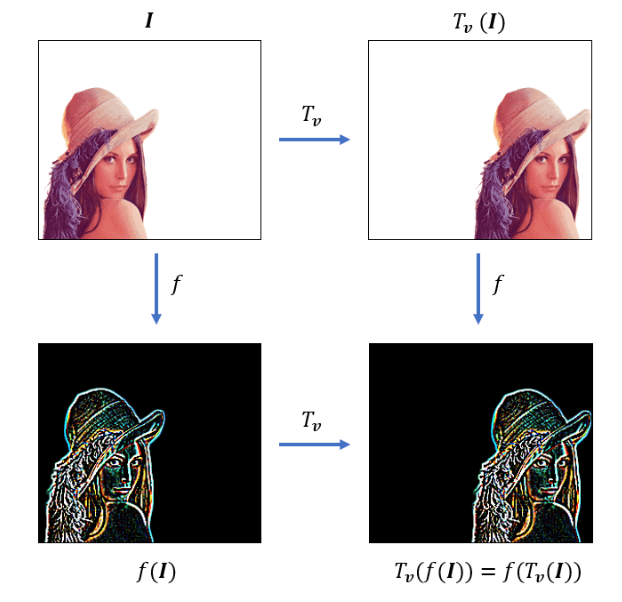
\includegraphics[width=0.5\textwidth]{../figures/equivariance.png}
    \end{center}
\end{frame}
%%%%%%%%%%%%%%%%%%%%%%%%%%%%%%%%%%%%%%%%%%%%%%%%%%%%%%%%%%%%%%%%%%%%%%%%%%%%%%



%%%%%%%%%%%%%%%%%%%%%%%%%%%%%%%%%%%%%%%%%%%%%%%%%%%%%%%%%%%%%%%%%%%%%%%%%%%%%%
\begin{frame}{Motivation}
    \begin{itemize}
        \setlength{\itemsep}{\fill}
        \item A cat is a cat no matter how you look at it.
    \end{itemize}

    \begin{center}
        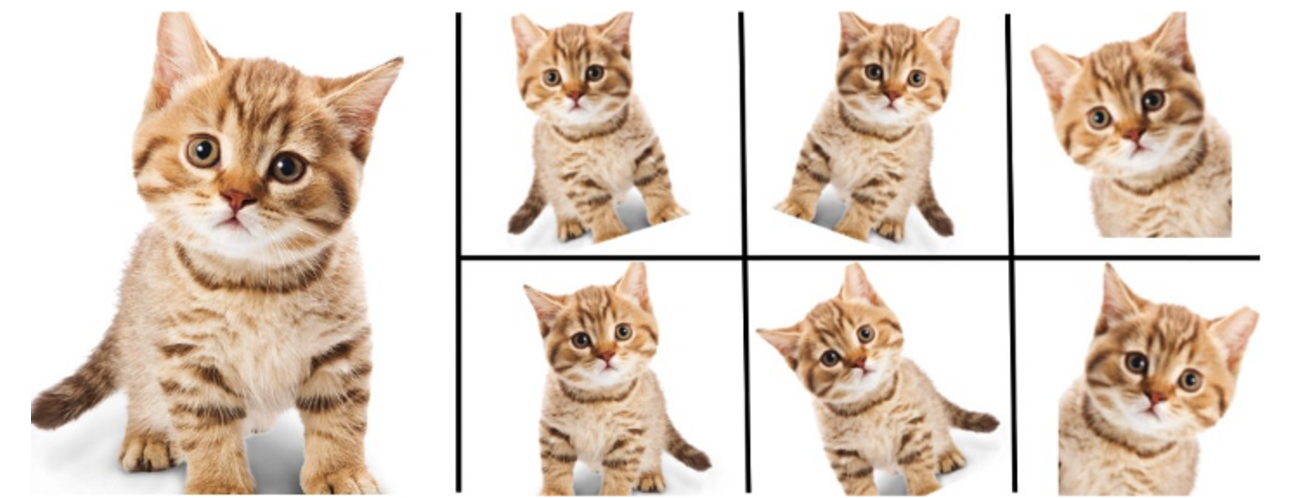
\includegraphics[width=0.8\textwidth]{../figures/cat.png}
    \end{center}

    \begin{itemize}
        \setlength{\itemsep}{\fill}
        \pause
        \item It is acceptable to assume that being invariant to the rotation of the cat is a good property for a classification network.
    \end{itemize}
\end{frame}
%%%%%%%%%%%%%%%%%%%%%%%%%%%%%%%%%%%%%%%%%%%%%%%%%%%%%%%%%%%%%%%%%%%%%%%%%%%%%%



%%%%%%%%%%%%%%%%%%%%%%%%%%%%%%%%%%%%%%%%%%%%%%%%%%%%%%%%%%%%%%%%%%%%%%%%%%%%%%
\begin{frame}{Motivation}
    \begin{itemize}
        \setlength{\itemsep}{\fill}
        \item Our focus today is on sets and graph data.
        \end{itemize}
    \begin{center}
        \begin{minipage}[t]{0.69\textwidth}
            \centering
            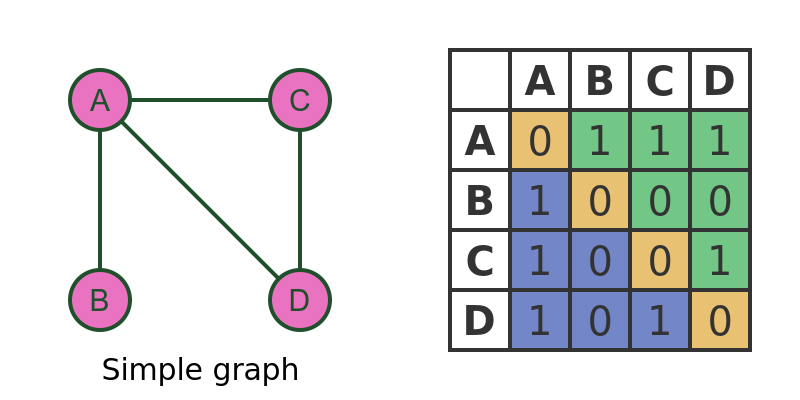
\includegraphics[width=\textwidth]{../figures/graph_adj.png}
        \end{minipage}
        \hfill
        \begin{minipage}[t]{0.3\textwidth}
            \centering
            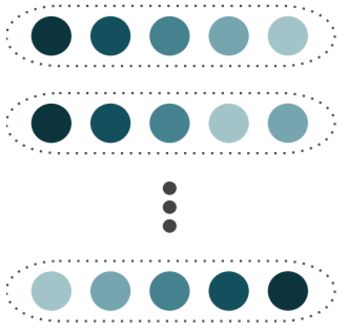
\includegraphics[width=\textwidth]{../figures/set.png}
        \end{minipage}
    \end{center}

\end{frame}
%%%%%%%%%%%%%%%%%%%%%%%%%%%%%%%%%%%%%%%%%%%%%%%%%%%%%%%%%%%%%%%%%%%%%%%%%%%%%%



%%%%%%%%%%%%%%%%%%%%%%%%%%%%%%%%%%%%%%%%%%%%%%%%%%%%%%%%%%%%%%%%%%%%%%%%%%%%%%

\section{Mathematical Backoground}

%%%%%%%%%%%%%%%%%%%%%%%%%%%%%%%%%%%%%%%%%%%%%%%%%%%%%%%%%%%%%%%%%%%%%%%%%%%%%%



%%%%%%%%%%%%%%%%%%%%%%%%%%%%%%%%%%%%%%%%%%%%%%%%%%%%%%%%%%%%%%%%%%%%%%%%%%%%%%
\begin{frame}{The Permutation Group $S_n$}

    \begin{itemize}
        \setlength{\itemsep}{\fill}
        \item The permutation group $S_n$ is the group of all permutations of $n$ elements.
        \item It has $n!$ elements, representing the $n!$ ways to order $n$ elements.
        \item Given a set $X = \{x_1, x_2, \ldots, x_n\}$, a permutation $\pi \in S_n$ is a bijection $\pi: X \rightarrow X$
        \item e.g. $x = (x_1, x_2, x_3)$, and $\pi = (1, 2, 3) \in S_3$ is the permutation that maps $1 \rightarrow 2$, $2 \rightarrow 3$ and $3 \rightarrow 1$.
        \item We denote the \textbf{action} of $\pi$ on $x$ as $\pi x = (x_3, x_1, x_2)$. 
    \end{itemize}
    
\end{frame}
%%%%%%%%%%%%%%%%%%%%%%%%%%%%%%%%%%%%%%%%%%%%%%%%%%%%%%%%%%%%%%%%%%%%%%%%%%%%%%



%%%%%%%%%%%%%%%%%%%%%%%%%%%%%%%%%%%%%%%%%%%%%%%%%%%%%%%%%%%%%%%%%%%%%%%%%%%%%%
\begin{frame}{Permutation Invariance}

    \begin{itemize}
        \setlength{\itemsep}{\fill}
        \item Let $H \leq S_n$ be a subgroup of the symmetric group.
        \pause
        \item $f:\mathbb{R}^n \rightarrow \mathbb{R}^n$ is permutation invariant if $f(x) = f(\pi x)$ for all $\pi \in H$.
    \end{itemize}
    \begin{center}
        \pause
        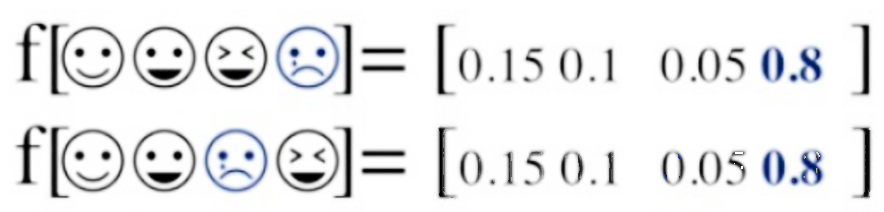
\includegraphics[width=0.65\textwidth]{../figures/perm_in.png}
    \end{center}
    
\end{frame}
%%%%%%%%%%%%%%%%%%%%%%%%%%%%%%%%%%%%%%%%%%%%%%%%%%%%%%%%%%%%%%%%%%%%%%%%%%%%%%



%%%%%%%%%%%%%%%%%%%%%%%%%%%%%%%%%%%%%%%%%%%%%%%%%%%%%%%%%%%%%%%%%%%%%%%%%%%%%%
\begin{frame}{Permutation Equivariance}

    \begin{itemize}
        \setlength{\itemsep}{\fill}
        \item Let $H \leq S_n$ be a subgroup of the symmetric group.
        \pause
        \item $f:\mathbb{R}^n \rightarrow \mathbb{R}^n$ is permutation invariant if $\pi f(x) = f(\pi x)$ for all $\pi \in H$.
    \end{itemize}
    \begin{center}
        \pause
        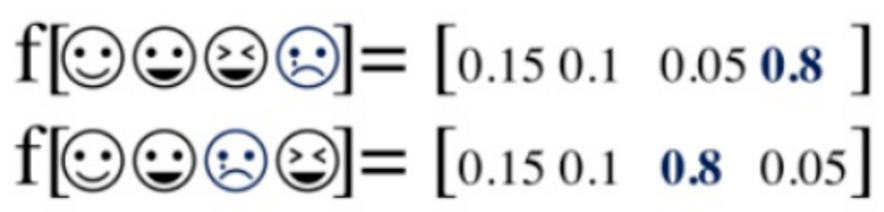
\includegraphics[width=0.65\textwidth]{../figures/perm_eq.png}
    \end{center}
    
\end{frame}
%%%%%%%%%%%%%%%%%%%%%%%%%%%%%%%%%%%%%%%%%%%%%%%%%%%%%%%%%%%%%%%%%%%%%%%%%%%%%%



%%%%%%%%%%%%%%%%%%%%%%%%%%%%%%%%%%%%%%%%%%%%%%%%%%%%%%%%%%%%%%%%%%%%%%%%%%%%%%
\begin{frame}{Permutation of a Set}

    \begin{itemize}
        \setlength{\itemsep}{\fill}
        \item Assume our set is $X = \{x_1, x_2, \ldots, x_n\}$.
        \pause
        \item We can represent $X$ as a matrix $X \in \mathbb{R}^{n \times d}$.
        \pause
        \item Any permutation $\pi \in S_n$ can be represented as a permutation matrix $\boldsymbol{P} \in \mathbb{R}^{n \times n}$,
        \pause
        \item The action of $\pi$ on $X$ is then $P X$.
        \pause
        \item An invariant neural network is a function $f: \mathbb{R}^{n \times d} \rightarrow \mathbb{R}^{d`}$ such that $f(X) = f(\boldsymbol{P}X)$.
        \pause
        \item An equivariant neural network is a function $f: \mathbb{R}^{n \times d} \rightarrow \mathbb{R}^{n \times d`}$ such that $\boldsymbol{P}f(X) = f(\boldsymbol{P}X)$.
    \end{itemize}
    
\end{frame}
%%%%%%%%%%%%%%%%%%%%%%%%%%%%%%%%%%%%%%%%%%%%%%%%%%%%%%%%%%%%%%%%%%%%%%%%%%%%%%


%%%%%%%%%%%%%%%%%%%%%%%%%%%%%%%%%%%%%%%%%%%%%%%%%%%%%%%%%%%%%%%%%%%%%%%%%%%%%%
\begin{frame}{Permutation of a Set}

    \begin{itemize}
        \setlength{\itemsep}{\fill}
        \item Our data is now a graph signal $(A, X) \in \mathbb{R}^{n \times n} \times \mathbb{R}^{n \times d}$. 
        \pause
        \item A permutation matrix $\boldsymbol{P} \in \mathbb{R}^{n \times n}$ acts on the adjacency matrix $A$ and the feature matrix $X$.
        \pause
        \item The action of $\boldsymbol{P}$ on $(A, X)$ is $(\boldsymbol{P^T}A\boldsymbol{P}, \boldsymbol{P}X)$.
    \end{itemize}
    
\end{frame}
%%%%%%%%%%%%%%%%%%%%%%%%%%%%%%%%%%%%%%%%%%%%%%%%%%%%%%%%%%%%%%%%%%%%%%%%%%%%%%



%%%%%%%%%%%%%%%%%%%%%%%%%%%%%%%%%%%%%%%%%%%%%%%%%%%%%%%%%%%%%%%%%%%%%%%%%%%%%%

\section{Invariant and Equivariant Construction}

%%%%%%%%%%%%%%%%%%%%%%%%%%%%%%%%%%%%%%%%%%%%%%%%%%%%%%%%%%%%%%%%%%%%%%%%%%%%%%



%%%%%%%%%%%%%%%%%%%%%%%%%%%%%%%%%%%%%%%%%%%%%%%%%%%%%%%%%%%%%%%%%%%%%%%%%%%%%%
\begin{frame}{Conclusion}
    \begin{itemize}
        \item end
    \end{itemize}
\end{frame}
%%%%%%%%%%%%%%%%%%%%%%%%%%%%%%%%%%%%%%%%%%%%%%%%%%%%%%%%%%%%%%%%%%%%%%%%%%%%%%



% Thank You Slide
\begin{frame}[plain]
    \centering
    \Huge Thank You!
\end{frame}

\end{document}
